% **************************************************************************************************************
% A Classic Thesis Style
% An Homage to The Elements of Typographic Style
%
% Copyright (C) 2007 Andr� Miede http://www.miede.de
%
% If you like the style then I would appreciate a postcard. My address
% can be found in the file ClassicThesis.pdf. A collection of the
% postcards I received so far is available online at
% http://postcards.miede.de
%
% License:
% This program is free software; you can redistribute it and/or modify
% it under the terms of the GNU General Public License as published by
% the Free Software Foundation; either version 2 of the License, or
% (at your option) any later version.
%
% This program is distributed in the hope that it will be useful,
% but WITHOUT ANY WARRANTY; without even the implied warranty of
% MERCHANTABILITY or FITNESS FOR A PARTICULAR PURPOSE.  See the
% GNU General Public License for more details.
%
% You should have received a copy of the GNU General Public License
% along with this program; see the file COPYING.  If not, write to
% the Free Software Foundation, Inc., 59 Temple Place - Suite 330,
% Boston, MA 02111-1307, USA.
%
% **************************************************************************************************************
% Note:
%    * You must not use "u etc. in strings/commands that will be spaced out (use \"u or real umlauts instead)
%    * Chapters must be marked with the \myChapter{Foo} command (sorry for the inconvenience at this point)
%    * New enumeration (small caps): \begin{aenumerate} \end{aenumerate}
%    * For margin notes: \graffito{}
%    * Do not use bold fonts in this style, it is designed around them
%    * Use tables as in the examples
%    * See classicthesis-ldpkg.sty for useful commands
% **************************************************************************************************************
% To Do:
%    * remove obsolete KOMA options and use \KOMAoptions instead
%    * support a List of Listings that looks like the other lists
% **************************************************************************************************************
%\documentclass[twoside,titlepage,fleqn,BCOR5mm]{scrbook}%,BCOR5mm

% Comentado por JCC 
\documentclass[10pt]{scrbook}%

%\usepackage[paperwidth=18.89cm,paperheight=24.58cm,twoside,bindingoffset=9mm,outer=2.2cm,inner=1cm,top=2.6cm,bottom=4.5cm]{geometry}

\let\upDelta\Delta
% ********************************************************************
% KOMA-Script setup (todo)
% ********************************************************************
\KOMAoptions{%
%    DIV=15,%
    BCOR=12mm,%
    %paper=b5,%
    fontsize=11pt,%
    cleardoublepage=empty,%
    headsepline=true,
    footinclude=true,%
    headinclude=true,%
    headlines=2.5,%
    open=right,%
    numbers=noenddot%
%    abstract=false%
}

\setlength{\paperwidth}{16.828cm} % set size for latex
\setlength{\paperheight}{26cm}
\special{papersize=16.828cm,26cm} % set size for ghostscript
\typearea[6mm]{1} % 6mm for spine

% ********************************************************************
% Development Stuff
% ********************************************************************
%\listfiles
%\usepackage[l2tabu, orthodox, abort]{nag}
%\usepackage[warning, all]{onlyamsmath}
% ********************************************************************
% Re-usable information
% ********************************************************************

% added by JCC to use Pygmentize 
% http://tex.stackexchange.com/questions/23458/how-to-install-syntax-highlight-package-minted-on-windows-7
% \newcommand\TestAppExists[3]{#2}
\usepackage{minted}


\newcommand{\myTitle}{INTELIGENCIA COMPUTACIONAL Y JUEGOS APLICADOS A LA ENSE\~NANZA\xspace}
\newcommand{\myDegree}{Doctor en Inform\'atica\xspace}
\newcommand{\myName}{Jos\'e Carpio Ca\~nada\xspace}
\newcommand{\myDegreeManualName}{Tesis Doctoral\xspace}
\newcommand{\myProf}{myProf\xspace}
\newcommand{\myOtherProf}{myOtherProf\xspace}
\newcommand{\myDirectorOne}{Juan Juli\'an Merelo Guerv\'os}
\newcommand{\myDirectorTwo}{V\'ictor Manuel Rivas Santos}
\newcommand{\myDirectorThree}{Alberto Prieto Espinosa}
\newcommand{\mySupervisor}{Prof. Dr. D. \myDirectorOne\\Prof. Dr. D. \myDirectorTwo}
\newcommand{\myFaculty}{Escuela T\'ecnica Superior de Inform\'atica y Telecomunicaciones\xspace}
\newcommand{\myDepartment}{Arquitectura y Tecnolog\'ia de Computadores\xspace}
\newcommand{\myDepartmentTwo}{Inform\'atica\xspace}
\newcommand{\myUni}{\protect{Universidad de Granada}\xspace}
\newcommand{\myUniTwo}{\protect{Universidad de Ja\'en}\xspace}
\newcommand{\myLocation}{Granada\xspace}
\newcommand{\myDay}{11}
\newcommand{\myTime}{Noviembre de 2014\xspace}

%*******************************************************
% Packages with options that might require adjustments
%*******************************************************
\usepackage[latin1]{inputenc}
\usepackage[spanish,ngerman,american,english,es-nodecimaldot]{babel}
\usepackage[square,numbers,sort&compress]{natbib}
\usepackage[spanish]{babelbib}
\usepackage[T1]{fontenc}
\usepackage{textcomp}
\usepackage[mathcal]{euscript}
\usepackage{latexsym}
\usepackage{relsize}
%\usepackage{amsmath} %Incompatible con \usepackage{relsize}
\usepackage{amsfonts}
\usepackage{amssymb}
%\usepackage[sort]{cite}
\usepackage[right]{eurosym}
\usepackage[top]{mcaption}
\usepackage[margincaption]{sidecap}

\usepackage{colortbl}
\usepackage{multirow}
\usepackage{rotating}

\usepackage{lettrine}
\usepackage{textcase}

\usepackage{url}
\usepackage{caption}
\usepackage[tight,spanish]{minitoc}

\usepackage{calc}
\usepackage{fp}

\usepackage{pgfplots}
\usetikzlibrary{dateplot}

\usepackage{cmap}

\usepackage{ifthen}

\usepackage{fancyvrb} %FERGU
\usepackage{etex}
\usepackage{minted}
\usepackage{algorithmic}
\providecommand{\e}[1]{\ensuremath{\times 10^{#1}}}

%\usepackage[a4,frame,center]{crop} %,cross

\input{coloricos} %OJO CON ESTO (EVOSOFT) vs highlight.sty de SOA-SOCO
\usepackage[final]{listings}


% JCC
\usepackage{color}
\pagecolor{white}
\usepackage[final]{pdfpages}

%\lstset{
%basicstyle=\ttfamily \scriptsize,
%backgroundcolor=\color{ultralightOrange},
%language=c++,
%frame=single,
%stringstyle=\ttfamily,
%showstringspaces=false
%} %DENTRO DE ESO HAY OTRO LISTINGS QUE SE COME LO DE ARRIBA, PERO NO SE SI AFECTA OTRAS COSAS...
%*******************************************************
\usepackage{classicthesis-ldpkg}
%*******************************************************
% Options for classicthesis.sty:
% tocaligned eulerchapternumbers drafting linedheaders listsseparated
% subfigure nochapters beramono eulermath parts minionpro pdfspacing
\usepackage[pdfspacing,eulerchapternumbers,crownquartopaper,%drafting,%linedheaders,%tocaligned,%
            subfigure,beramono,eulermath,parts]{classicthesis2}
% ********************************************************************
% Language/strings for backrefs (change here, thanks, Lorenzo)
%*******************************************************
\renewcommand{\backrefnotcitedstring}{\relax}%(Not cited.)
%\renewcommand{\backrefcitedsinglestring}[1]{(Citado en la p\'agina~#1.)}
%\renewcommand{\backrefcitedmultistring}[1]{(Citado en las p\'aginas~#1.)}
%\renewcommand{\backreftwosep}{ y~}
%\renewcommand{\backreflastsep}{ y~}
% ********************************************************************
% Setup and Finetuning
%*******************************************************
\newlength{\abcd} % for ab..z string length calculation
\newcommand{\myfloatalign}{\centering} % how all the floats will be aligned
\setlength{\extrarowheight}{3pt} % increase table row height
% ********************************************************************
% Captions look and feel
%*******************************************************
\DeclareCaptionFont{titlecolor}{\color{titlecolor}\fontfamily{pbk}\selectfont}
\DeclareCaptionFont{alternateTitlecolor}{\color{alternateTitlecolor}\fontfamily{pbk}\selectfont}
\captionsetup{justification=RaggedRight,format=plain,labelsep=newline,font=scriptsize,labelfont=titlecolor,textfont=alternateTitlecolor}%
% ********************************************************************
% Where to look for graphics
%*******************************************************
%\graphicspath{{gfx/}{misc/}} % considered harmful according to l2tabu
% ********************************************************************
% Hyperreferences
%*******************************************************
\hypersetup{%
    colorlinks=true, linktocpage=true, pdfstartpage=3, pdfstartview=FitV,%
    breaklinks=true, pdfpagemode=UseNone, pageanchor=true, pdfpagemode=UseOutlines,%
    plainpages=false, bookmarksnumbered, bookmarksopen=true, bookmarksopenlevel=1,%
    hypertexnames=true, pdfhighlight=/O,%hyperfootnotes=true,%nesting=true,%frenchlinks,%
    urlcolor=colorCorporativoOscuro, linkcolor=alternateTitlecolor, citecolor=Maroon, %pagecolor=RoyalBlue,%
    % uncomment the following line if you want to have black links (e.g., for printing)
    %urlcolor=Black, linkcolor=Black, citecolor=Black, %pagecolor=Black,%
    pdftitle={\myTitle},%
    pdfauthor={\textcopyright\ \myName, \myUni, \myFaculty},%
    pdfsubject={},%
    pdfkeywords={},%
    pdfcreator={pdfLaTeX},%
    pdfproducer={LaTeX with hyperref and classicthesis}%
}
%********************************************************************
% Hyphenation
%*******************************************************
%\hyphenation{Mul-ti-pli-ca-ti-ve de-sa-rro-llar he-te-ro-g�-ne-os pro-pues-ta o-fi-ci-na vi-de-o-ga-mes zoo-kee-per sub-po-pu-la-tion pa-ra-digm Sprin-ger Mi-guel Mo-ra ha-bi-ta-ci�n I-lle-ras Ge-ne-bot pre-sents Ba-ye-sian al-go-rithms E-C-F re-pla-cer re-pla-cer-Na-me He-Ha OS-Gi OS-Gi-Liath W-S-D-L pro-vi-der M-M-D-P}


%********************************************************************
% Redefinir en espa�ol la edici�n en la bibliograf�a
%*******************************************************

\declarebtxcommands{spanish}{%
\def\btxnumeralshort#1{%
${#1}^a$}%\btxnumeralfallback{spanish}{#1}}%
\def\btxnumerallong#1{%
${#1}^a$}%\btxnumeralfallback{spanish}{#1}}%
}

%********************************************************************
% Renombrar al espa�ol algunos identificadores
%*******************************************************

%\renewcommand{\contentsname}{Lista de Contenidos}
%\renewcommand{\listfigurename}{Lista de Figuras}
%\renewcommand{\listtablename}{Lista de Tablas}
%\renewcommand{\bibname}{Bibliograf�a}
%\renewcommand{\partname}{Parte}
%\renewcommand{\figurename}{Figura}
%\renewcommand{\tablename}{Tabla}
%\newcommand{\tablaname}{Tabla}
%\renewcommand{\cfttabpresnum}{\tablaname~}

\renewcommand{\person}[1]{{\color{Maroon}{#1}}}

\selectbiblanguage{spanish}

%\renewcommand{\spacedallcaps}[1]{\textsc{\MakeTextUppercase{#1}}}
%\renewcommand{\spacedlowsmallcaps}[1]{\textsc{\MakeTextUppercase{#1}}}

%********************************************************************
% Tipos de letras
%*******************************************************

%\renewcommand{\encodingdefault}{T1}
%\renewcommand{\familydefault}{gm}%papyrus}%bradley} %pbk,ppl
%\renewcommand{\seriesdefault}{b}

%\renewcommand{\rmdefault}{bradley}

\newcommand{\Copyright}{{\small$^\mathrm{\copyright}$}~}
\newcommand{\apriori}{\emph{a priori}\xspace}
\newcommand{\aposteriori}{\emph{a posteriori}\xspace}
\newcommand{\etal}{\emph{et al.}\xspace}
\newcommand{\cronbach}{\mbox{$\alpha$--\emph{Cronbach}}\xspace}

\newcommand{\itemlabel}[1]{{\color{Maroon}{\textsc{#1}}}}

\newcommand{\mysize}{\tiny}

%********************************************************************
% Colores
%*******************************************************

%\definecolor[named]{ultralightOrange}{rgb}{1,.94,.72}
%\definecolor[named]{highlightOrange}{rgb}{1,.86,.29}
%\definecolor[named]{lightOrange}{rgb}{1,.45,0}
\definecolor[named]{darkOrange}{rgb}{.8,.3,0}

\definecolor[named]{minimumOrange}{rgb}{1,.976,.474}
\definecolor[named]{ugrOrange}{rgb}{.945,.365,.165} % PANTONE 179: {R:241, G:93, B:42}
%\definecolor[named]{ugrOrange}{cmyk}{0,.309,.368,0} % PANTONE 179: {C:0, M:79, Y:94, K:0}
\definecolor[named]{ugrGray}{rgb}{.463,.482,.494}

%\definecolorseries{ugrOrangeSerie}{rgb}{last}{ugrOrange}{white}
%\resetcolorseries[10]{ugrOrangeSerie}

\colorlet{ultralightOrange}{ugrOrange!5!minimumOrange}
\colorlet{highlightOrange}{ugrOrange!25!minimumOrange}
\colorlet{lighterOrange}{ugrOrange!40!minimumOrange}
\colorlet{lightOrange}{ugrOrange!75!minimumOrange}

\definecolor{colorCorporativoMasSuave}{named}{ultralightOrange}
\definecolor{colorCorporativoSuave}{named}{highlightOrange}
\definecolor{colorCorporativoMedioSuave}{named}{lighterOrange}
\definecolor{colorCorporativoMedio}{named}{lightOrange}
\definecolor{colorCorporativo}{named}{ugrOrange}
\definecolor{colorCorporativoOscuro}{named}{darkOrange}
\definecolor{Maroon}{named}{colorCorporativoOscuro}

\definecolor{headColor}{named}{white}%{colorCorporativoMasSuave}
\definecolor{titleNumbercolor}{named}{ugrGray}
\definecolor{titlecolor}{named}{ugrOrange}
\definecolor{alternateTitlecolor}{named}{darkOrange}

\newcolumntype{A}{%
>{\color{black}\columncolor{colorCorporativoSuave}}%
p{0.95\textwidth}}

\newcolumntype{B}{%
>{\color{black}\columncolor{colorCorporativoMasSuave}}%
p{0.95\textwidth}}

\newcolumntype{C}{%
>{\columncolor{colorCorporativoSuave}}p{\textwidth}}
%>{\columncolor{colorCorporativo}}p{4pt}}

\newcolumntype{D}{%
>{\color{black}\fontfamily{pbk}\selectfont\columncolor{colorCorporativoSuave}}p{8em}}
%>{\columncolor{colorCorporativo}}p{4pt}

%********************************************************************
% Cabeceras
%*******************************************************

\def\ptctitle{Index}
\def\mtctitle{Index}
\def\stctitle{Index}
\setlength{\mtcindent}{0pt}
\renewcommand{\mtifont}{\normalsize\scshape\lsstyle}

%\typearea[current]{last}
%\typearea[current]{current}
%\setlength{\topmargin}{-4em}
%\setlength{\textheight}{590.80026pt}%{595.80026pt}
%\setlength{\tabcolsep}{1em}




\newboolean{TesisCompleta}
\setboolean{TesisCompleta}{false}

\newboolean{PaginasDeInicio}
\setboolean{PaginasDeInicio}{true}

\newcounter{IncluyeCapitulo}
\setcounter{IncluyeCapitulo}{2}


% ********************************************************************
% ********************************************************************
% ********************************************************************
% Comienza el documento
% ********************************************************************
% ********************************************************************
% ********************************************************************
\begin{document}
\frenchspacing
\raggedbottom
%\selectlanguage{spanish}
%\renewcommand{\contentsname}{Lista de Contenidos}
%\renewcommand{\listfigurename}{Lista de Figuras}
%\renewcommand{\listtablename}{Lista de Tablas}
%\renewcommand{\bibname}{Bibliograf�a}
%\renewcommand{\partname}{Parte}
%\renewcommand{\figurename}{Figura}
%\renewcommand{\tablename}{Tabla}
%\renewcommand{\figureautorefname}{Figura}
%\renewcommand{\tableautorefname}{Tabla}
%\renewcommand{\paragraphautorefname}{P\'arrafo}
%\renewcommand{\subparagraphautorefname}{Subp\'arrafo}
%\renewcommand{\footnoteautorefname}{Nota al pie}
%\renewcommand{\FancyVerbLineautorefname}{}
%\renewcommand{\theoremautorefname}{Teorema}
%\renewcommand{\appendixautorefname}{Ap\'endice}
%\renewcommand{\equationautorefname}{Ecuaci\'on}
%\renewcommand{\itemautorefname}{Item}
%\newcommand*{\subfigureautorefname}{Figura}

% Par�metros para Lettrine (lo de la primera letra m�s grande en los comienzos de los cap�tulos)
%
\setcounter{DefaultLines}{2}
\renewcommand{\DefaultLoversize}{0.1} %0.25
\renewcommand{\DefaultLraise}{0.3} %0.25
\renewcommand{\DefaultLhang}{0.5} %0.5
\setlength{\DefaultFindent}{0pt}%0.5em}
\setlength{\DefaultNindent}{0pt}%0.1em}
\setlength{\DefaultSlope}{0pt}
\renewcommand{\LettrineFontHook}{\color{colorCorporativoOscuro}\fontfamily{fau}}%{fau}pzc}\fontseries{bx}\fontshape{it}}
\renewcommand{\LettrineTextFont}{\color{colorCorporativoOscuro}\fontfamily{fau}\scshape}

\pagenumbering{roman}
\pagestyle{scrheadings}%{plain}

\renewcommand{\labelenumii}{\arabic{enumii}.}

%********************************************************************
% Definiciones Captions
%*******************************************************

\sidecaptionvpos{figure}{t}

\ifthenelse{\boolean{PaginasDeInicio}}{
%********************************************************************
% Frontmatter
%*******************************************************
% \include{FrontBackmatter/DirtyTitlepage}
\pagecolor{white}
%*******************************************************
% Signed Titlepage 
%*******************************************************
\begin{titlepage}
    \begin{center}
        \large
        \vspace*{1.5cm}
        \includegraphics[width=8cm]{gfx/ugr_formal} \\

        \vspace{1.5cm}

        {\color{ugrOrange}\spacedallcaps{\myTitle}} \\ \bigskip
	{\textcolor{ugrGray} {\small Presentado por}} \\ \bigskip
        \spacedlowsmallcaps{\myName}

        \vspace{1.5cm}
\textcolor{ugrGray}
        {\small To apply for the }\normalsize\\
        \large\spacedlowsmallcaps{International PhD Degree in} \\ 
        \large\spacedlowsmallcaps{Computer and Network Engineering} \\
\vspace{1.5cm}
\textcolor{ugrGray}{\small Directores }\normalsize\\
        \large\spacedlowsmallcaps{\myDirectorOne}\\
        \large\spacedlowsmallcaps{\myDirectorTwo}\\
        \vspace{3cm}

        {\small Firmado: \myName }\\ \bigskip
	Noviembre 2014


    \end{center}
\end{titlepage}   
%\include{FrontBackmatter/Titlepage}
\include{FrontBackmatter/Titleback}
\cleardoublepage
%%*******************************************************
% Signed Titlepage 
%*******************************************************
\begin{titlepage}
    \begin{center}
        \large
        \vspace*{1.5cm}
        \includegraphics[width=8cm]{gfx/ugr_formal} \\

        \vspace{1.5cm}

        {\color{ugrOrange}\spacedallcaps{\myTitle}} \\ \bigskip
	{\textcolor{ugrGray} {\small Presentado por}} \\ \bigskip
        \spacedlowsmallcaps{\myName}

        \vspace{1.5cm}
\textcolor{ugrGray}
        {\small To apply for the }\normalsize\\
        \large\spacedlowsmallcaps{International PhD Degree in} \\ 
        \large\spacedlowsmallcaps{Computer and Network Engineering} \\
\vspace{1.5cm}
\textcolor{ugrGray}{\small Directores }\normalsize\\
        \large\spacedlowsmallcaps{\myDirectorOne}\\
        \large\spacedlowsmallcaps{\myDirectorTwo}\\
        \vspace{3cm}

        {\small Firmado: \myName }\\ \bigskip
	Noviembre 2014


    \end{center}
\end{titlepage}   

%\cleardoublepage
%*******************************************************
% Declaration
%*******************************************************
\refstepcounter{dummy}
\pdfbookmark[1]{Visto Bueno}{Visto Bueno}
\chapter*{Visto Bueno}
\thispagestyle{empty}
\bigskip

%\noindent\textit{\myLocation, \myTime}

\vfil

El \textbf{Prof. Dr. D. \myDirectorOne}, Catedr�tico de Universidad del Departamento de \myDepartment de la \myUni y el profesor \textbf{Prof. Dr. D. \myDirectorTwo}, Titular de Universidad del Departamento de \myDepartmentTwo de la \myUniTwo,

\bigskip

\textsc{certifican:}

\bigskip

\noindent Que la memoria titulada:
\begin{center}
``\textbf{\emph{\myTitle}}''
\end{center}
ha sido realizada por \textbf{D. \myName} bajo nuestra direcci�n en el Departamento de \myDepartment de la \myUni para optar al grado de \textbf{\myDegree}.

\vfil

\begin{center}
En \myLocation, a \myDay\xspace de \myTime.
\end{center}
\vfil
Los Directores de la tesis doctoral:\\
\vspace{2cm}

\begin{center}
Fdo. \myDirectorOne \\ y \myDirectorTwo \\
\end{center}

% \begin{flushright}
%     \begin{tabular}{m{5cm}}
%         \\ \hline
%         \centering\myName \\
%     \end{tabular}
% \end{flushright}

\cleardoublepage
%*******************************************************
% Declaration
%*******************************************************
\refstepcounter{dummy}
\pdfbookmark[1]{Declaraci�n}{Declaraci�n}
\chapter*{Declaraci�n}
\thispagestyle{empty}
\vfill

\noindent El doctorando \myName y los directores de la tesis \myDirectorOne y \myDirectorTwo \xspace garantizamos, al firmar esta tesis doctoral, que el trabajo ha sido realizado por el doctorando bajo la direcci�n de los directores de la tesis y hasta donde nuestro conocimiento alcanza, en la realizaci�n del trabajo, se han respetado los derechos de otros autores a ser citados, cuando se han utilizado sus resultados o publicaciones.  
\smallskip


\bigskip

\noindent\textit{\myLocation, \myTime}

\bigskip
\bigskip
\bigskip

\begin{flushright}
    \begin{tabular}{m{3cm}m{7cm}}
        & \\ \hline
        \centering\myName & \myDirectorOne \newline y \myDirectorTwo
    \end{tabular}
\end{flushright}

\vfill
\cleardoublepage
%*******************************************************
% Dedication
%*******************************************************
\thispagestyle{empty}
%\phantomsection
\refstepcounter{dummy}
\pdfbookmark[1]{Dedicatoria}{Dedicatoria}

\vspace*{3cm}

\begin{flushright}
A mi familia: \hspace{3em}\\
Manuel Angel, Matilde, Manuel Jos�, Fernando, Lolita y Elisa Matilde.\\
\end{flushright}



\medskip

\cleardoublepage
%*******************************************************
% Abstract
%*******************************************************
%\renewcommand{\abstractname}{Abstract}
\pdfbookmark[1]{Abstract}{Abstract}
\begingroup
\let\clearpage\relax
\let\cleardoublepage\relax
\let\cleardoublepage\relax



\pdfbookmark[1]{Abstract}{Abstract}
\chapter*{Abstract}

% The objective of this thesis is to prove that the Service Oriented Architecture (SOA) paradigm can be used to create distributed, heterogeneous, dynamic and standards-based environments for Evolutionary Algorithms (EAs). SOA provides independence in programming language and transmission mechanisms, and also facilitates  dynamic component management. 

% A methodology to develop EAs in these environments is proposed. In this methodology, called SOA-EA, the SOA paradigm is proposed to develop Service Oriented Evolutionary Algorithms (SOEAs).  The proposed methodology takes into account the requirement to develop services and EAs, and it provides the steps to identify, specify, implement and deploy the elements that conform a SOEA, and how to convert a traditional EA into a SOEA. To validate this methodology, it has been used to create a framework for SOEAs, called OSGiLiath, based in a public specification technology (OSGi). This framework provides mechanisms for dynamic component management and language and transmission independence. 

% OSGiLiath and SOA-EA have been used to carry out experiments in different areas to validate dynamic control and different and heterogeneous environments: decentralized distributed EAs, other systems integration and different EA models.


\chapter*{Resumen}
%Esta Tesis Doctoral trata de probar que usar un marco determinado es
%el m�s adecuado para solucionar problemas actuales en los Algoritmos

% aparte de que no se entiende, est� mal: usar un marco... es el m�s
% adecuado �Qu� marco? �Sabes cu�l? �Lo vas a buscar en la tesis? �Vas
% a comparar varios marcos? Si lo sabes de antemano, di cual y por qu�
% a priori debe ser el m�s adecuado - JJ
%Evolutivos en desarrollo, integraci�n, interoperabilidad y
%dinamismo. Para validar este objetivo la tesis se ha dividido en 3
%partes.  
% Yo quitar�a desarrollo; para desarrollar los lenguajes de script son
% m�s f�ciles - JJ

%Primero se analizan las nuevas tendencias % las tendencias no se
                                % analizan, se hallan. �Esto d�nde lo
                                % haces? Ten en cuenta que toda la
                                % tesis debe de ir a avanzar estos
                                % tres objetivos, y *debes decirlo
                                % expl�citamente* - JJ
%en investigaci�n en Algoritmos Evolutivos para detectar sus principales carencias y se propone el uso de Arquitectura Orientada a Servicios (AOS) como el marco para resolver estas carencias.

%La siguiente parte de esta tesis propone una metodolog�a (SOA-EA) para
%desarrollar Algoritmos Evolutivos Orientados a Servicios (AEOS). Esta
%metodolog�a se ha utilizado para implementar un framework para AEOS,
%llamado OSGiLiath, utilizando una tecnolog�a concreta (OSGi). Se
%presentan diferentes experimentos para validar cada una de las mejoras
%propuestas. % �Qu� mejoras? �El objetivo de la tesis son esas mejoras?
            % No has mencionado ni una vez si has tenido que hacer un
            % cambio en el algoritmo ni si has propuesto un nuevo
            % algoritmo. �La adaptaci�n de los AGs a OSGi es directa?
            % Si es as�, es s�lo implementaci�n y no hay mucha
            % tesis. �Tienen m�s enjundia?

%OSGiLiath se ha usado tambi�n para desarrollar un m�todo para adaptar
%el tama�o de poblaci�n de un AE distribuido a la potencia de calculo
%de los nodos que forman el sistema distribuido. Finalmente, SOA-EA y
%OSGiLiath se han utilizado en otras aplicaciones: generaci�n de un bot
%inteligente para un juego en tiempo real y arte generativo. % �Eh? �Se
                                % ha usado tambi�n? �Te pillaba de
                                % camino? �Es parte de la tesis? �Es
                                % consecuencia de la tesis? �La
                                % prueba? �En esas aplicaciones se
                                % prueba que es el m�s guay o te
                                % pillaban de camino? - JJ

%Esto es lo que deber�as haber escrito para empezar y no perderlo
%nunca de vista. �C�mo puedes escribir la tesis si no sabes lo que
%pretende? - JJ FERGU: estaba en el github, pero lo pongo aqu� (luego lo traduzco cuando tenga el visto bueno)

\vfill

% No me gusta nada este resumen. No abarca toda la tesis (no abarca
% las aplicaciones ni las encaja m�s que con un "tambi�n". 
%FERGU: reescrito abajo entero

% El objetivo de esta tesis es demostrar que el paradigma de Arquitectura Orientada a Servicios (AOS) puede usarse para crear entornos distribuidos, heterog�neos, din�micos y basados en est�ndares para Algoritmos Evolutivos (AEs). AOS proporciona independencia en el lenguaje de programaci�n y mecanismo de transmisi�n y facilita la administraci�n de componentes de forma din�mica. 

% Se propone crear una metodolog�a para desarrollar AEs en estos entornos. En esta metodolog�a, denominada SOA-EA, se propone el uso del paradigma de SOA para desarrollar Algoritmos Evolutivos Orientados a Servicios (AEOS).  La metodolog�a propuesta tiene en cuenta los requisitos para desarrollar servicios y EAs y proporciona los pasos para identificar, especificar, implementar y desplegar los componentes que forman un AEOS, y c�mo convertir un AE tradicional a un AEOS. Para validarla, esta metodolog�a se ha utilizado para crear un framework para AEOS, llamado OSGiLiath, basado una tecnolog�a p�blica (OSGi). Este framework  proporciona mecanismos para administraci�n de componentes din�micos, independencia del lenguaje y protocolo de comunicaci�n. 

% Tanto OSGiLiath como SOAEA se han utilizado para realizar experimentos en distintos campos para validar el control del dinamismo y la heterogeneidad: AEs distribuidos no centralizados, integraci�n con otros sistemas y distintos modelos de EAs.

\endgroup

\vfill
\cleardoublepage
% JCC
% %*******************************************************
% Publications
%*******************************************************
\pdfbookmark[1]{Publications}{Scientific Publications}
\chapter*{Scientific Publications}
Some of the ideas, images and data exposed in this thesis have been previously published in the next references:
\bigskip

\begin{itemize}
% \item \person{Pablo Garc�a-S�nchez, J. Gonz�lez, Pedro A. Castillo, Maribel Garc�a Arenas, Juan Juli�n Merelo Guerv�s} \emph{Service oriented evolutionary algorithms}.  Soft Comput. 17(6): 1059--1075 (2013).


% no metas estos del "companion", que todos sabemos lo que es... 

% \item \person{Pablo Garc�a-S�nchez, Maria I. Garc�a Arenas, Antonio Miguel Mora, Pedro A. Castillo, Carlos Fernandes, Paloma de las Cuevas, Gustavo Romero, Jes�s Gonz�lez, Juan Juli�n Merelo Guerv�s} \emph{ Developing services in a service oriented architecture for evolutionary algorithms}. In Proceeding of the fifteenth annual conference companion on Genetic and evolutionary computation conference companion. ACM, 2013. p: 1341-1348.

% \item \person{Pablo Garc�a-S�nchez} \emph{ A service oriented evolutionary architecture: applications and results}. In Proceeding of the fifteenth annual conference companion on Genetic and evolutionary computation conference companion. ACM, 2013. p: 1663--1666.

% \item \person{Pablo Garc�a-S�nchez, J. Gonz�lez, Pedro A. Castillo, Juan Juli�n Merelo Guerv�s, Antonio Miguel Mora, Juan Lu�s Jim�nez Laredo, Maribel Garc�a Arenas} \emph{ A Distributed Service Oriented Framework for Metaheuristics Using a Public Standard}. In Proceeding of Nature Inspired Cooperative Strategies for Optimization. Studies in Computational Intelligence. Springer, 2010. p: 211--222.


% \item \person{P. Garc�a-S�nchez, A. Fern�ndez-Ares, A. M. Mora, P. A. Castillo, J. Gonz�lez and J.J. Merelo} \emph{Tree depth influence in Genetic Programming for generation of competitive agents for RTS games}. Applications of Evolutionary Computation, EvoApplicatons 2010: EvoCOMPLEX, EvoGAMES, EvoIASP, EvoINTELLIGENCE, EvoNUM, and EvoSTOC, Proceedings. Springer, 2014. Lecture Notes in Computer Science (to appear).

% \item \person{P. Garc�a-S�nchez, A. M. Mora, P. A. Castillo, J. Gonz�lez and J.J. Merelo} \emph{A methodology to develop Service Oriented Evolutionary Algorithms}. Proceedings of 8th International Symposium on Intelligent Distributed Computing (IDC'2014) Springer, 2014. Studies in Computational Science (to appear).

\end{itemize}

\cleardoublepage
%*******************************************************
% Acknowledgments
%*******************************************************
\pdfbookmark[1]{Agradecimientos}{agradecimientos}

\begin{flushright}
 
\end{flushright}



\bigskip

\begingroup
\let\clearpage\relax
\let\cleardoublepage\relax
\let\cleardoublepage\relax
\chapter*{Agradecimientos}
Mis agradecimientos van en primer lugar a mi familia Manuel Jos�, Matilde, Manuel �ngel, Fernando, Lola y Elisa que son las ramitas que dan fuerza 
y sentido a la vida.
A JJ y V�ctor, por su paciencia, por dejar que me equivocase tantas veces y sobre todo por haber sido capaces de darme la �ltima oportunidad despu�s
 de tantas anteriores.   
A Nicol�s, Carmen, Alicia, Nico y Eloy que ha sido mi segunda familia durante las estancias en el CITIC por su apoyo, sus risas matutinas, sus consejos
 y sus maravillosas cenas.
A mis compa�eros de Geneura que me acompa�aron en este largo viaje JJ, V�ctor, Pedro, Gustavo, Pablo, Juanlu, Antonio Mora, Maribel, Paloma, Antares a
 los que espero poder devolver alg�n d�a todo lo que me han dado. A mis compa�eros de Huelva, Nacho, Miguel �ngel, Fran, Gonzalo, Manuel, Manuel Emilio, 
 Manolo Vasallo, Teresa, Jos� Luis �lvarez, Jos� Luis Arjona, Paco M�rquez, Patricia, I�aki, Nieves, Antonio Peregr�n, Manolo Redondo, Javier Aroba por
 las maravillosas charlas sobre temas cient�ficos y no cient�ficos. A Jos� Manuel And�jar por apostar por mi desde el principio y por dejarme meter la
 pata. A los compa�eros de Simple LAB Juan Diego, Manuel, Miguel �ngel, Juan Manuel Enrique y Antonio por tanta energ�a e ilusi�n puesta en los nuevos
 proyectos. A la gente de CRM y en especial a Antonio Palanco y su familia por estar siempre dispuesto a echar un cable para lo que sea. 
A Carmen, Cristina, Fernando y todos los que colaboraron en hacer que la FLL se celebrase en Huelva por primera y segunda vez.   
A los compa�eros y personal del CITIC por hacer de ese espacio un hogar para muchos investigadores.  Al Dr. Tom�s Mateo Sanguino sin cuyo trabajo y tes�n
 no hubiese sido posible esta tesis. Al Dr. Arturo Aquino, por sus sabios consejos, su apoyo y su amistad. A Jos� Enrique Cano por su amistad y por
 ense�arme a dedicarme con pasi�n a descubrir, sea en el �mbito que sea. A mis amigos Nicol�s, Nico, Alejandro, Javi Aguayo, Jes�s, Alex, Dani y al 
 resto de la familia de Tarifa, Andy, Samuel, Silvia, Amparo, Lidia, Marcos Benavent, Felipe y tantos otros que fueron, siguen siendo y ser�n un gran
 apoyo tanto en lo profesional como en lo personal.
A mis alumnos, los que participaron en competiciones y art�culos cient�ficos y a los que no, por ser una pieza tan importante en el d�a a d�a y a quienes
 en especial va dedicado este trabajo.
"Si est�s leyendo esto cerca de m� y no te he nombrado es que soy un desastre y merezco que me des una colleja ... Gracias a todos. Por cierto, si est�s
 leyendo esto y no te conozco quiere decir que te interesa esta tesis, as� que te la dedico a ti tambi�n, qu� demonios." Gracias Pablo por la frase, no 
 he visto una mejor forma de terminar esta secci�n.
 

\endgroup




\pagestyle{scrheadings}
\cleardoublepage
%*******************************************************
% Table of Contents
%*******************************************************
%\phantomsection
\refstepcounter{dummy}
\pdfbookmark[1]{\contentsname}{tableofcontents}
\setcounter{tocdepth}{2}
\dominitoc
\tableofcontents
%\markboth{\spacedlowsmallcaps{\contentsname}}{\spacedlowsmallcaps{\contentsname}}
\markboth{\textsc{\contentsname}}{\textsc{\contentsname}}
%*******************************************************
% work-around to have small caps also here in the headline
% will not work at this place if the TOC has more than 2 pages
% use \manualmark and then the \markboth as above
% later a modification of \automark[section]{chapter}
%*******************************************************
% List of Figures and of the Tables
%*******************************************************
\clearpage

\begingroup
    \let\clearpage\relax
    \let\cleardoublepage\relax
    \let\cleardoublepage\relax
    %*******************************************************
    % List of Figures
    %*******************************************************
    %\phantomsection
    \refstepcounter{dummy}
    %\addcontentsline{toc}{chapter}{\listfigurename}
    \pdfbookmark[1]{\listfigurename}{lof}
    \listoffigures

    \vspace*{8ex}

    %*******************************************************
    % List of Tables
    %*******************************************************
    %\phantomsection
    \refstepcounter{dummy}
    %\addcontentsline{toc}{chapter}{\listtablename}
    \pdfbookmark[1]{\listtablename}{lot}
    \listoftables

    \vspace*{8ex}
%   \newpage

    %*******************************************************
    % List of Listings
    %*******************************************************
%   %\phantomsection
%   \refstepcounter{dummy}
%   %\addcontentsline{toc}{chapter}{\lstlistlistingname}
%   \pdfbookmark[1]{\lstlistlistingname}{lol}
%   \lstlistoflistings

    %*******************************************************
    % Acronyms
    %*******************************************************
    %\phantomsection
    \refstepcounter{dummy}
    \pdfbookmark[1]{Acronyms}{acronyms}
    \chapter*{Acr\'onimos}
    \begin{acronym}[CSCW]
    \acro{CI}{Computational Intelligence}
    \acro{API}{Application Programming Interface}
    \acro{CPU}{Central Processing Unit}
	\acro{EA}{Evolutionary Algorithm}
    \acro{EC}{Evolutionary Computation}
    \acro{EP}{Evolutionary Programming}
	\acro{ES}{Evolutionary Strategy}
    \acro{GA}{Genetic Algorithm}
    \acro{GP}{Genetic Programming}
    \end{acronym}
\endgroup

\cleardoublepage 
}
{

}



% *******************************************************
% Mainmatter
% *******************************************************
\pagenumbering{arabic}

\ifthenelse{\boolean{TesisCompleta}}{
%-----------------------------
\myPart{Introducción}\label{part:introduccion}

%REALMENTE tienes que escribir una introducción. 

}
{
%-----------------------------  PONER LETTRINE EN SECCIONES Y NO INDENT EN SUBSECCIONES!!!
% -- \myPart{Introduction}\label{part:introduccion}

%----- Modificado por JCC
% -- \ifthenelse{\equal{\value{IncluyeCapitulo}}{2}}{\include{Chapters/00-intro}}{\myChapter{Introduction}\label{chap:introduction}}
% -- \ifthenelse{\equal{\value{IncluyeCapitulo}}{2}}{\include{Chapters/00-intro-SPANISH}}{\myChapter{Introducci{\'o}n}\label{chap:introductionSPANISH}}
% --\ifthenelse{\equal{\value{IncluyeCapitulo}}{2}}{\include{Chapters/02-distributedEAs}}{\myChapter{Evolutionary Algorithms}\label{chap:distributedEAs}}

%-----------------------------
% -- \myPart{Materials and Methods}\label{part:metodoYmateriales}
% -- \ifthenelse{\equal{\value{IncluyeCapitulo}}{2}}{\include{Chapters/03-soa}}{\myChapter{Service Oriented Architecture: technologies and restrictions for designing services for EAs}\label{chap:soa}}
% -- \ifthenelse{\equal{\value{IncluyeCapitulo}}{2}}{\include{Chapters/04-soaea}}{\myChapter{A methodology for developing services for EAs}\label{chap:soaea}}
%-----------------------------
% -- \myPart{Experimental Results}\label{part:resultadosExperimentales}
% -- \ifthenelse{\equal{\value{IncluyeCapitulo}}{2}}{\include{Chapters/05-osgiliath}}{\myChapter{Implementation of SOA-EA}\label{chap:osgiliath}}
% -- \ifthenelse{\equal{\value{IncluyeCapitulo}}{2}}{\include{Chapters/06-adaptive}}{\myChapter{Parameter adaptation in heterogeneous machines}\label{chap:adaptive}}
%\ifthenelse{\equal{\value{IncluyeCapitulo}}{2}}{\include{Chapters/07-art}}{\myChapter{HSV and RGB comparison in Evolutionary Art}\label{chap:art}}
% -- \ifthenelse{\equal{\value{IncluyeCapitulo}}{2}}{\include{Chapters/08-rts}}{\myChapter{Generation of bots for RTS games using Genetic Programming}\label{chap:rts}}

%-----------------------------
% -- \myPart{Conclusions}\label{part:discusionYconclusiones}
% -- \ifthenelse{\equal{\value{IncluyeCapitulo}}{2}}{\include{Chapters/09-conclusions}}{\myChapter{Conclusions and future work}\label{chap:conclusions}}
% -- \ifthenelse{\equal{\value{IncluyeCapitulo}}{2}}{\include{Chapters/09-conclusions-SPANISH}}{\myChapter{Conclusiones y trabajo futuro}\label{chap:conclusionsSPANISH}}
%\ifthenelse{\equal{\value{IncluyeCapitulo}}{12}}{\include{Chapters/conclusiones}}{\myChapter{Conclusiones}\label{chap:conclusiones}}

}


% *******************************************************
% Backmatter
% *******************************************************
\appendix
\myPart{Appendix}
% \include{Chapters/appendixosgi}
% \include{Chapters/appendixosgiliath}

% JCC PDFs
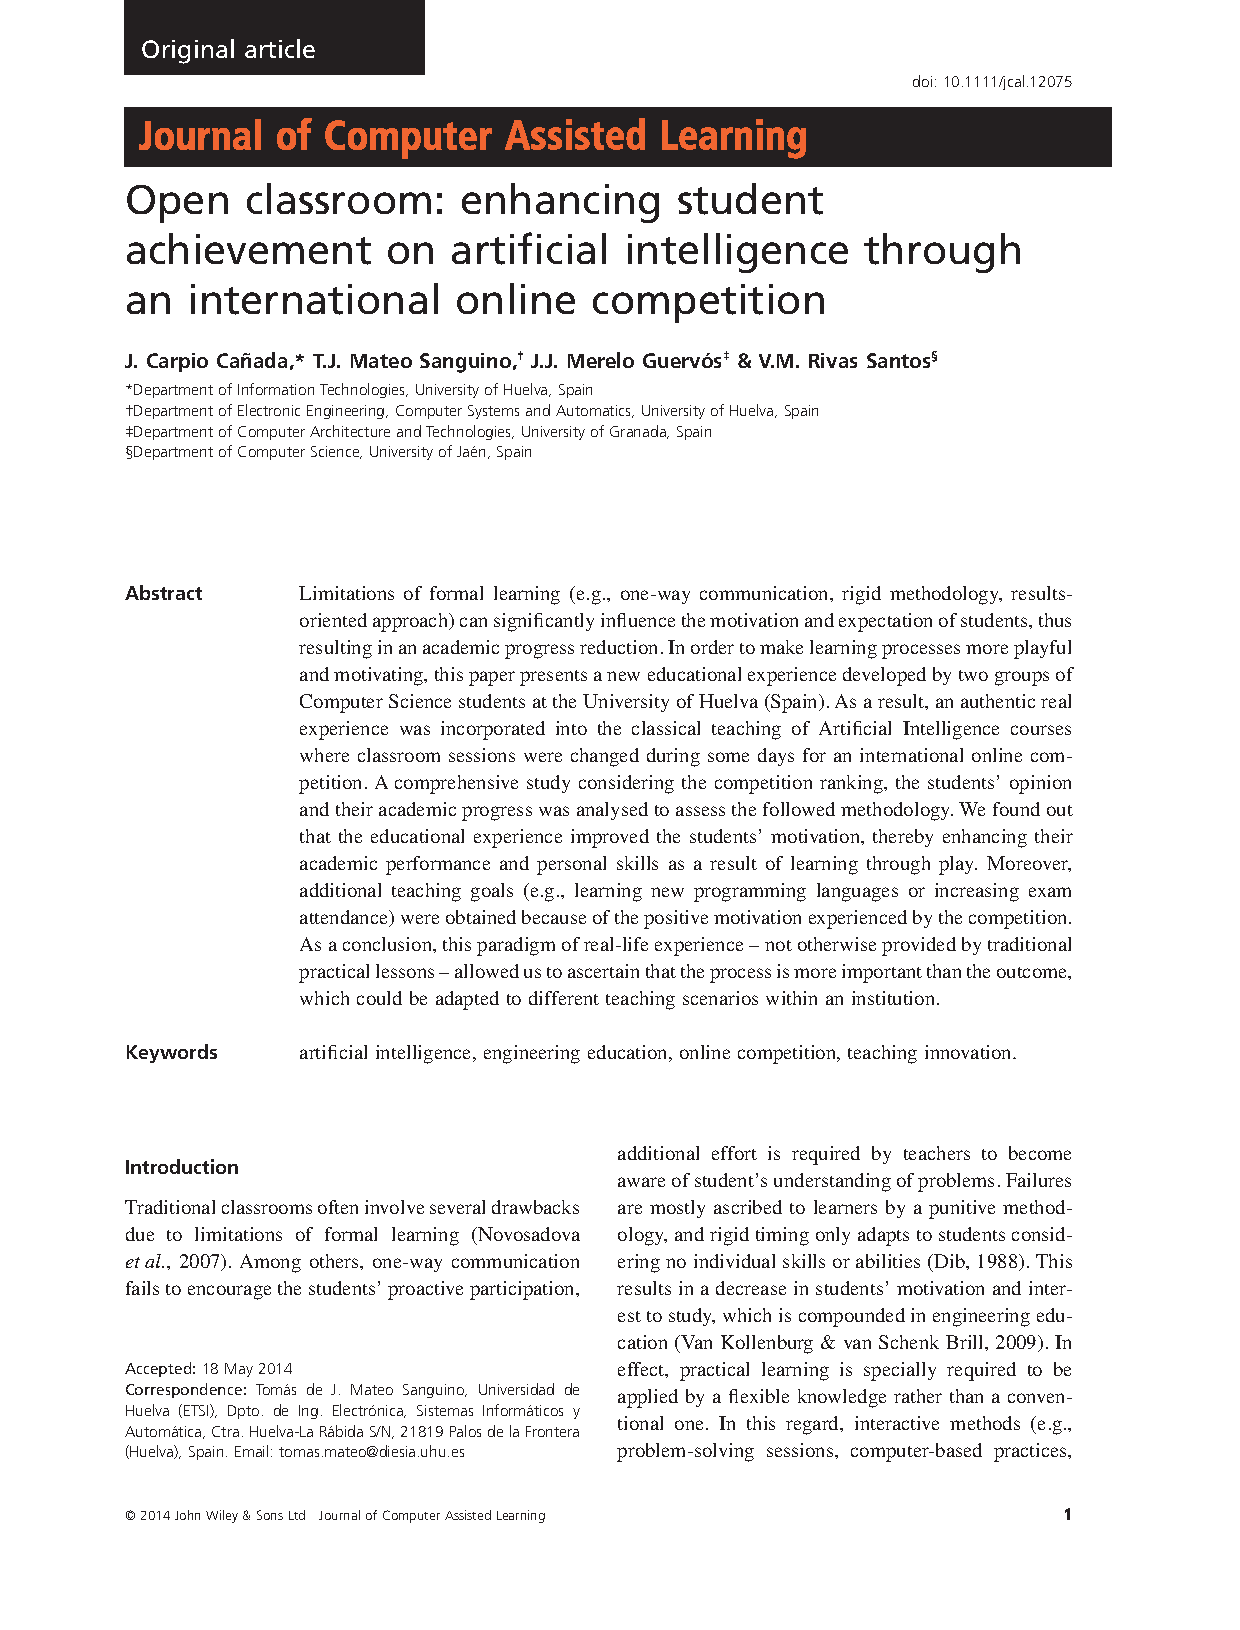
\includepdf[pages={-},scale=1.0,pagecommand={},offset=-0.5cm -0.5cm,
 addtolist={1, table, {Evolving Multilayer Perceptrons}, tab:evolving}]{pdf/jcal12075.pdf}
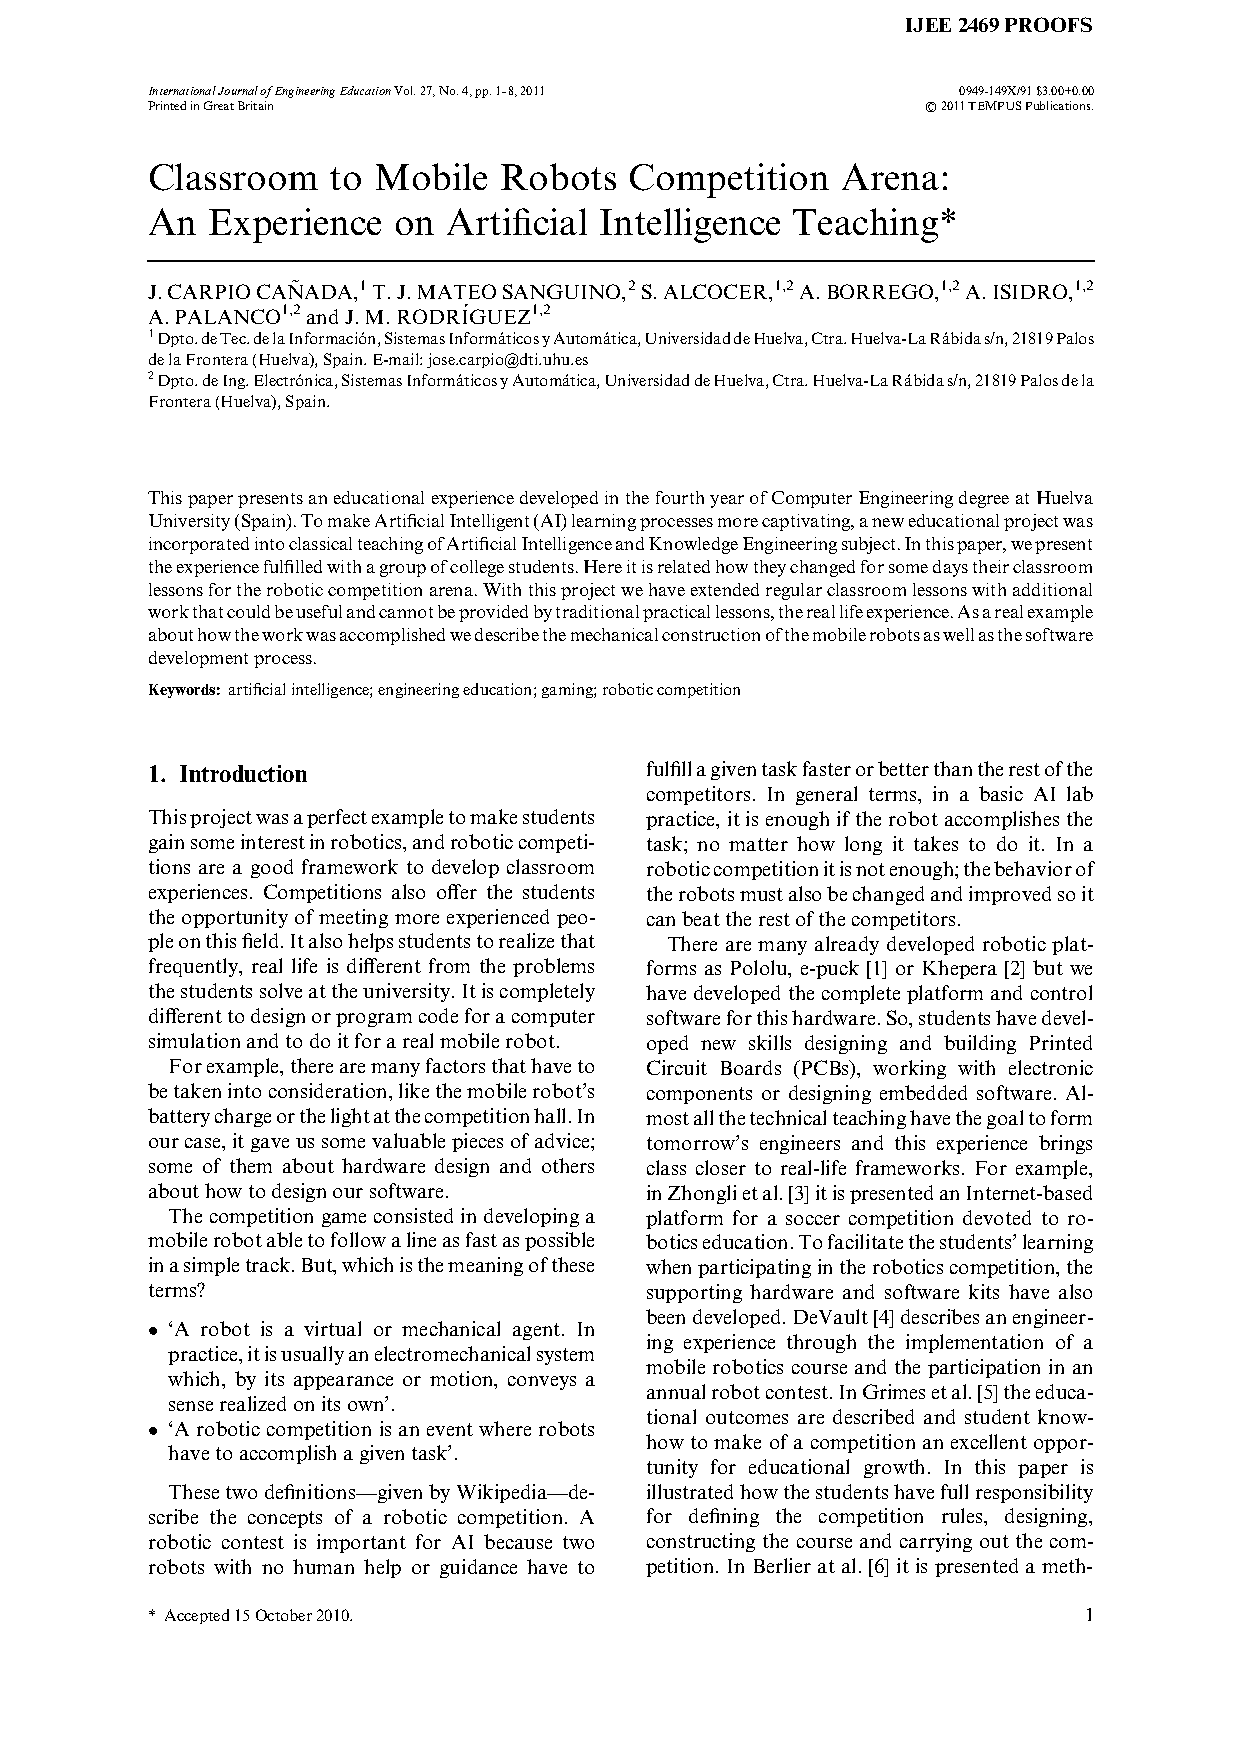
\includepdf[pages={-},scale=1.0,pagecommand={},offset=-0.5cm -0.5cm,
 addtolist={1, table, { Classroom to Mobile Robots Competition Arena: An experience on AI Teaching}, tab:robots}]{pdf/ijee2469ns.pdf}
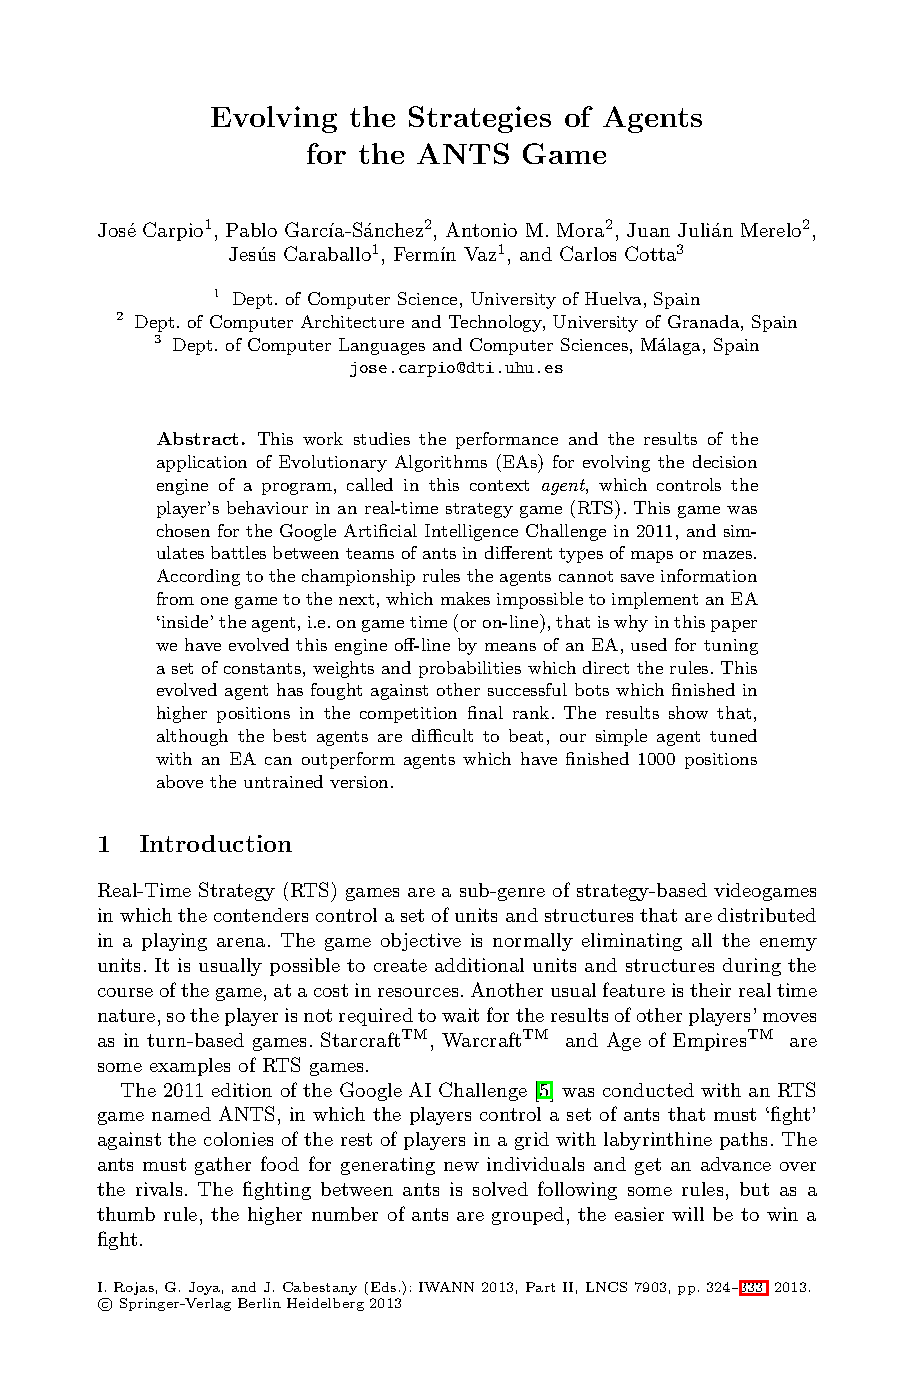
\includepdf[pages={-},scale=1.0,pagecommand={},offset=-0.5cm -0.5cm,
 addtolist={1, table, {Open classroom: enhancing student achievement on AI through an international online computation }, tab:cosmobot}]{pdf/ants_iwann2013.pdf}
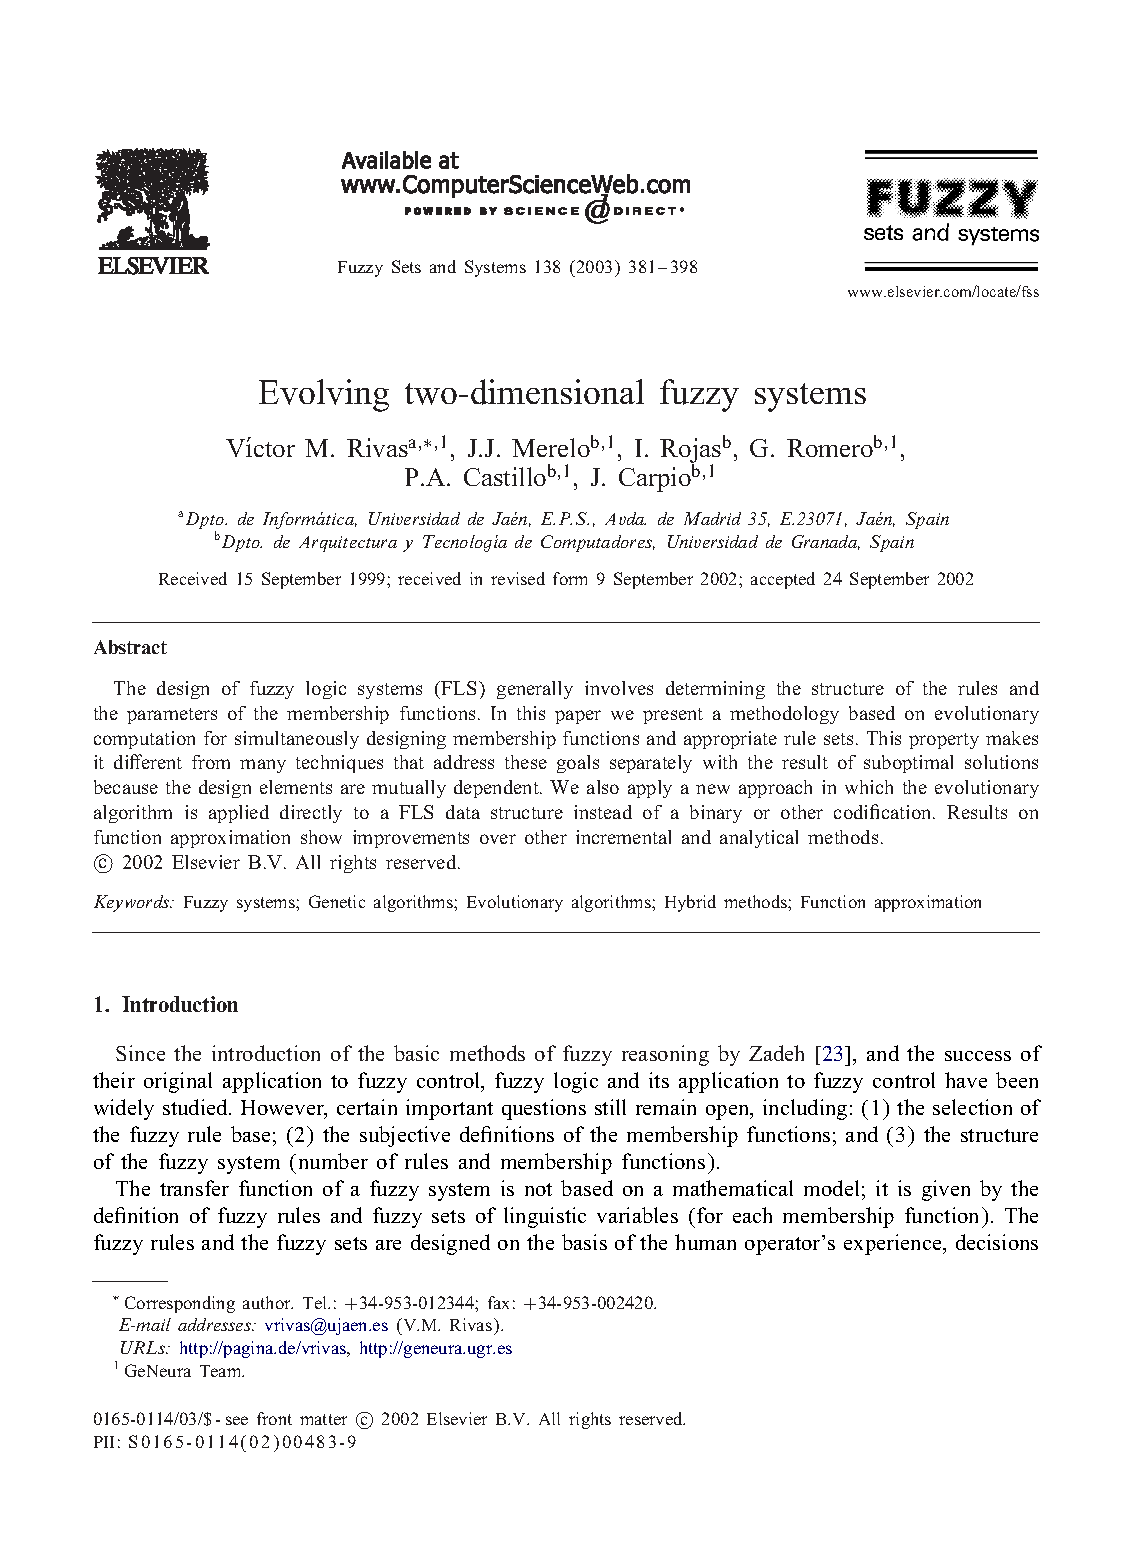
\includepdf[pages={-},scale=1.0,pagecommand={},offset=-0.5cm -0.5cm,
 addtolist={1, table, {Evolving the Strategies of Agents for the ANTS Game}, tab:iwann}]{pdf/evolving.pdf}


% 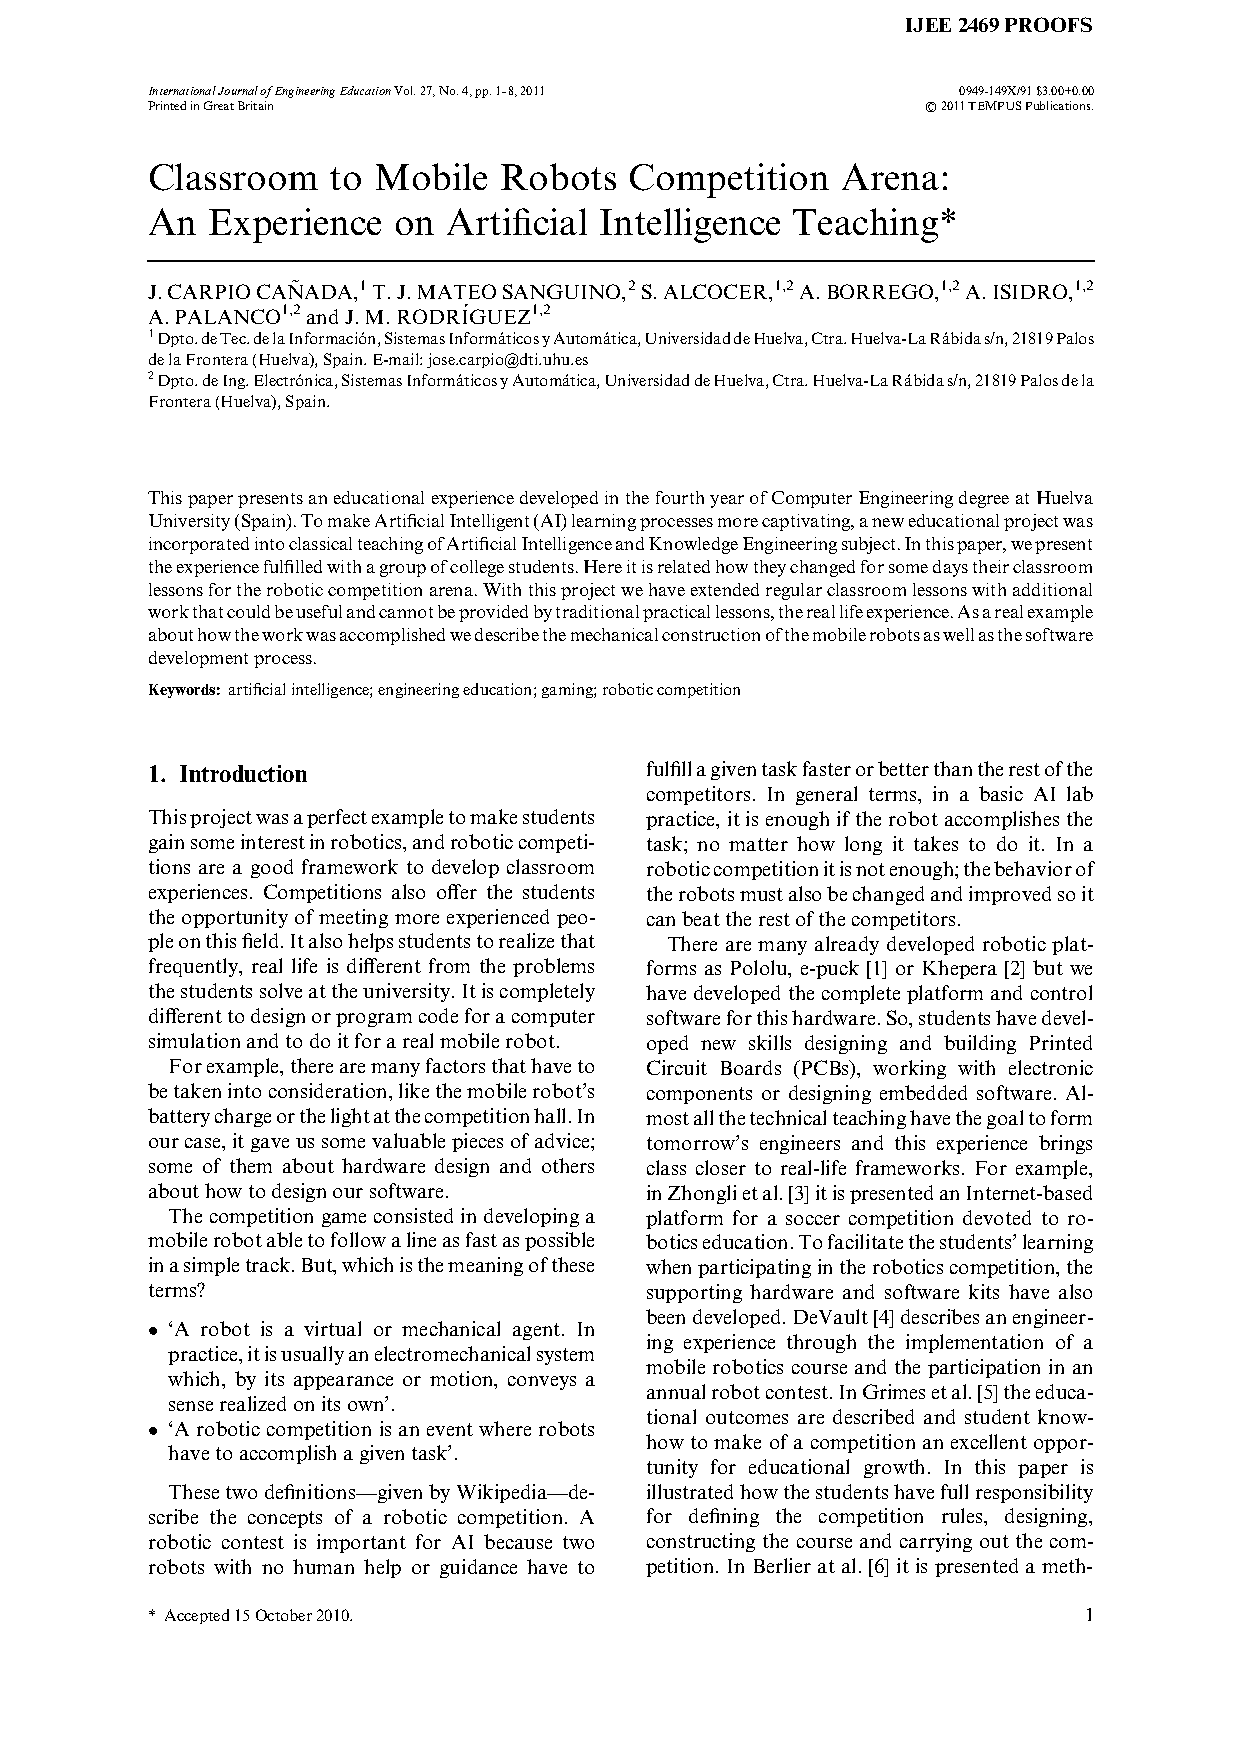
\includepdf[pages={-}]{pdf/ijee2469ns.pdf}
% 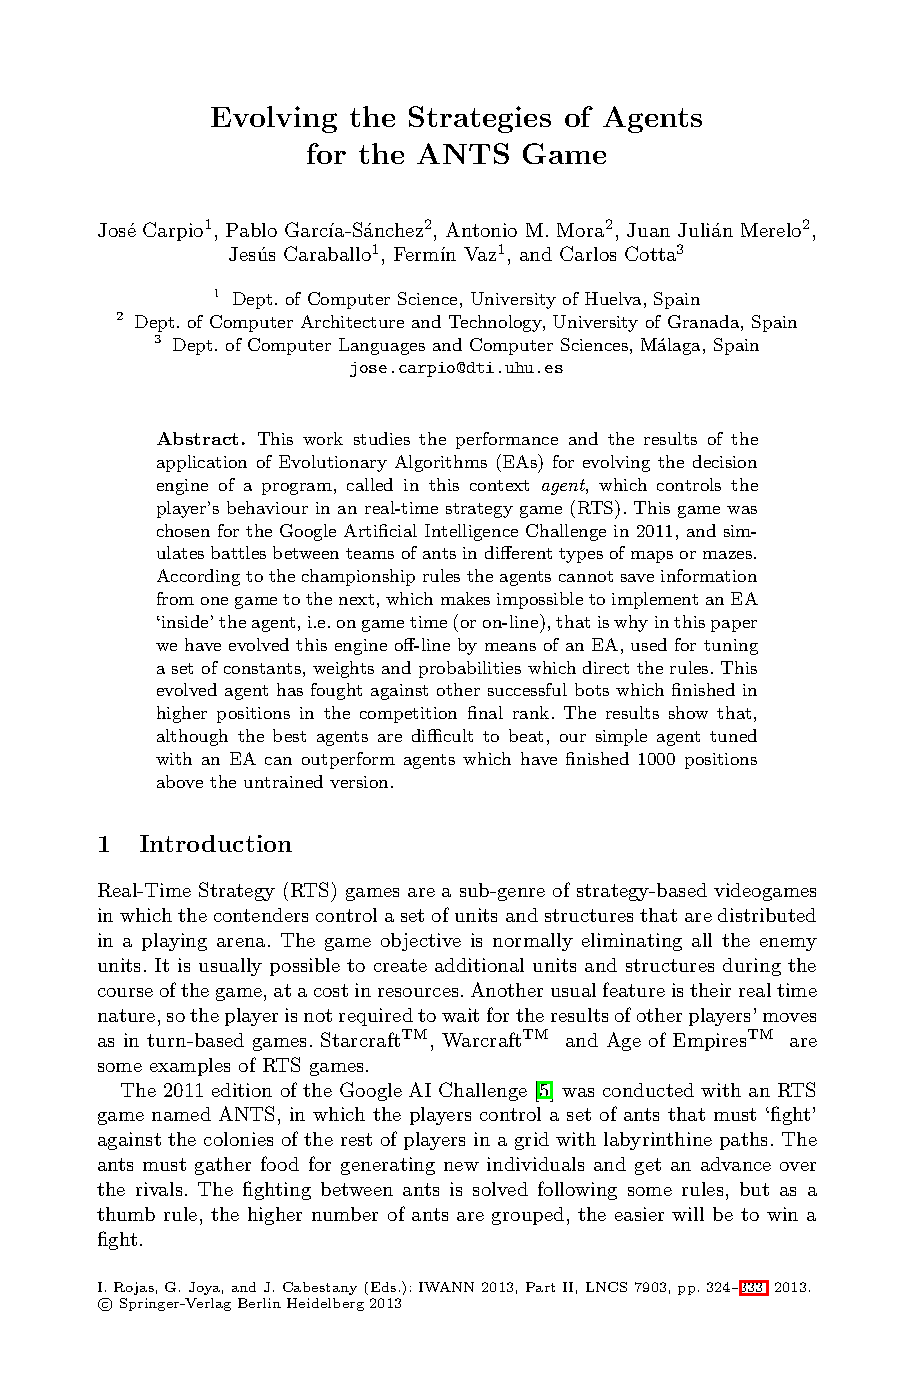
\includepdf[pages={-}]{pdf/ants_iwann2013.pdf}
% 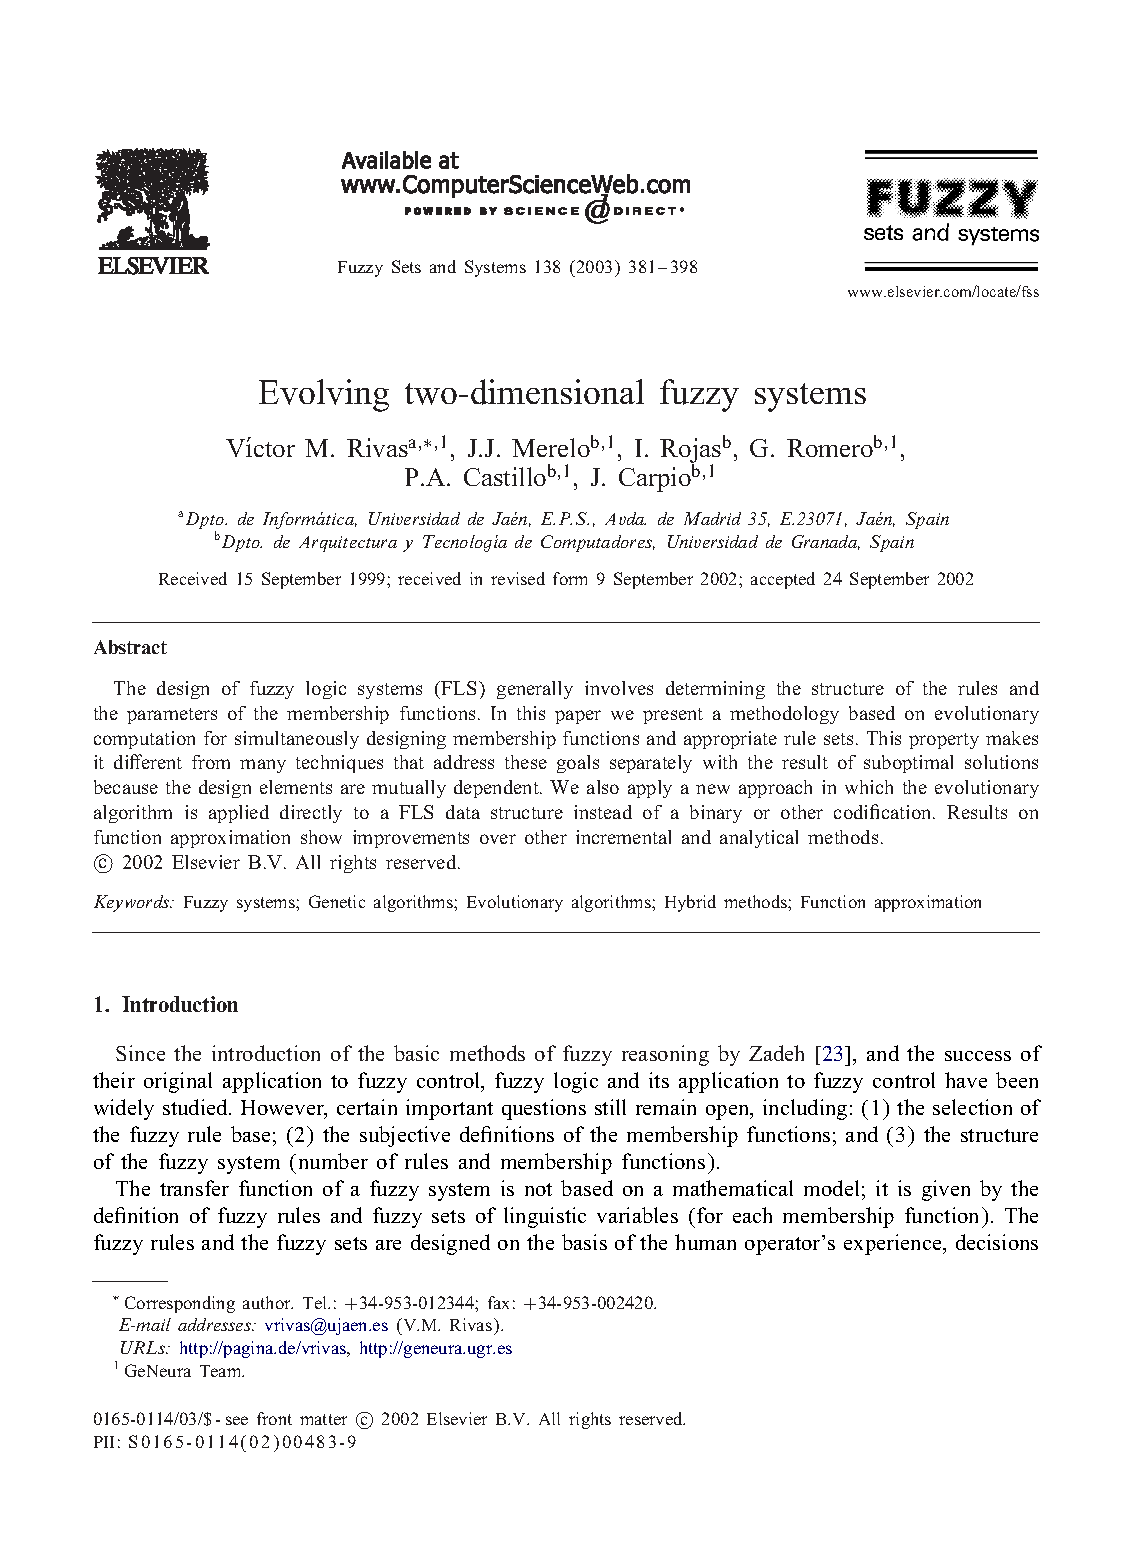
\includepdf[pages={-}]{pdf/evolving.pdf}

%\include{Chapters/apendiceC}
%********************************************************************
% Other Stuff in the Back
%*******************************************************
\cleardoublepage
%********************************************************************
% Bibliography
%*******************************************************
% work-around to have small caps also here in the headline
\pdfbookmark[0]{\bibname}{\bibname}

% \manualmark
% \markboth{\spacedlowsmallcaps{\bibname}}{\spacedlowsmallcaps{\bibname}} % work-around to have small caps also
%\phantomsection
\refstepcounter{dummy}
\addtocontents{toc}{\protect\vspace{\beforebibskip}} % to have the bib a bit from the rest in the toc
\addcontentsline{toc}{chapter}{\tocEntry{\bibname}}
%\bibliographystyle{plainnat}
\bibliographystyle{babplain-fl}
\label{app:bibliography}
\bibliography{tesis} 
%\cleardoublepage
%%*******************************************************
% Declaration
%*******************************************************
\refstepcounter{dummy}
\pdfbookmark[1]{Declaraci�n}{Declaraci�n}
\chapter*{Declaraci�n}
\thispagestyle{empty}
\vfill

\noindent El doctorando \myName y los directores de la tesis \myDirectorOne y \myDirectorTwo \xspace garantizamos, al firmar esta tesis doctoral, que el trabajo ha sido realizado por el doctorando bajo la direcci�n de los directores de la tesis y hasta donde nuestro conocimiento alcanza, en la realizaci�n del trabajo, se han respetado los derechos de otros autores a ser citados, cuando se han utilizado sus resultados o publicaciones.  
\smallskip


\bigskip

\noindent\textit{\myLocation, \myTime}

\bigskip
\bigskip
\bigskip

\begin{flushright}
    \begin{tabular}{m{3cm}m{7cm}}
        & \\ \hline
        \centering\myName & \myDirectorOne \newline y \myDirectorTwo
    \end{tabular}
\end{flushright}

\vfill
\cleardoublepage
%La contraportada tiene que estar en página par!!
% \include{FrontBackmatter/DirtyBackpage}

% ********************************************************************
% Game Over: Restart, Restore or Quit?
%*******************************************************
\end{document}
% ********************************************************************
